%------------- Normal Forces at Feet -------------%
\subsection{Normal Forces at Feet}
\label{sec:normal_forces}

The normal forces acting on the robot are shown in Figure \ref{fig:robot_ext_fbd}. The 5 legged robot is considered a statically indeterminate (hyperstatic) case (as determined from the original equations shown in Appendix \ref{app:feet_force}). Thus it is impossible to mathematically determine the resulting force at every foot of the robot without considering bending in the robot's material. 

\begin{figure}[H]
    \centering
    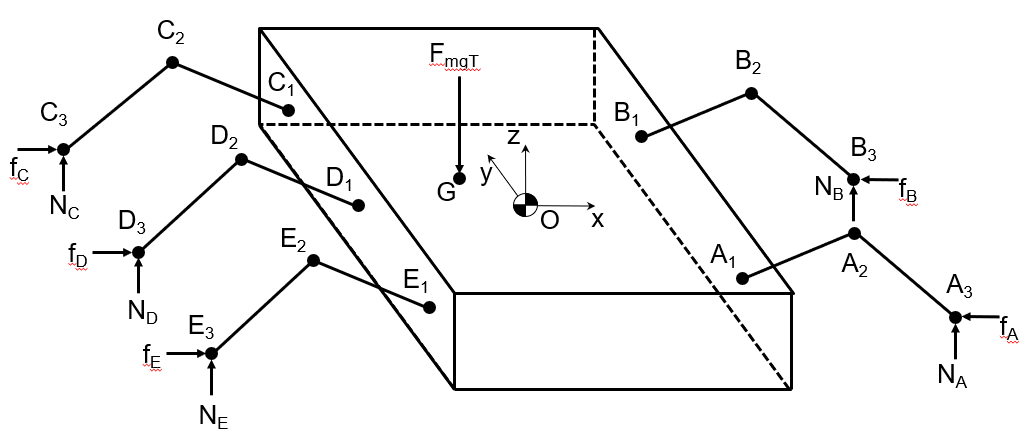
\includegraphics[width=\textwidth]{4_ComponentProperties/img/robot_ext_fbd.PNG}
    \caption{FBD of Whole Robot}
    \label{fig:robot_ext_fbd}
\end{figure}

In order to calculate realistic (worst case) values of torque, the reaction forces at the robot's feet were calculated for two possible solutions where only three feet would touch the ground. 

The 2 combinations of feet touching the ground are: 1. A, C, D and 2. B, D, E. To simplify calculations and algebra, a matrix system approach was used. 

For combination 1., the sum of forces and moments are given by
\begin{gather}
    \sum F_z = 0 = N_A + N_C + N_D - F_{mgT}
    \\
    \sum M_{A_x} = 0 = N_C r_{ca_y} + N_D r_{da_y} - F_{mgT} r_{ga_y}
    \\
    \sum M_{C_y} = 0 = -N_A r_{ac_x} -N_D r_{dc_x} + F_{mgT} r_{gc_x}
\end{gather}

For combination 2., the sum of forces and moments are given by
\begin{gather}
    \sum F_z = 0 = N_B + N_D + N_E - F_{mgT}
    \\
    \sum M_{B_x} = 0 = -N_D r_{db_y} - N_E r_{eb_y} + F_{mgT} r_{gb_y}
    \\
    \sum M_{E_y} = 0 = -N_B r_{be_x} -N_D r_{de_x} + F_{mgT} r_{ge_x}
\end{gather}

where the $r$ values represent the distance between the foot and the reference point, perpendicular to the rotation axis.

The following is an example with combination 1. A matrix solver is used to find reaction values.

\begin{equation}
\begin{split}
    \left[ \begin{array}{ccc} 
    N_A 
    \\ 
   N_C
    \\ 
    N_D
    \end{array} \right]= \left[ \begin{array}{ccc} 
    1 & 1 & 1 
    \\ 
    0 & r_{ca_y} & r_{da_y} 
    \\ 
    r_{ac_x} & r_{dc_x} & 0
    \end{array} \right]^{-1}
    \left[ \begin{array}{ccc} 
    F_{mgT}
    \\ 
    F_{mgT} r_{ga_y} 
    \\ 
    F_{mgT} r_{gc_x}
    \end{array} \right] 
    \\ 
   = \left[ \begin{array}{ccc} 
    1 & 1 & 1 
    \\ 
    0 & 600 mm & 200mm 
    \\ 
    1624mm & 0 & 0
    \end{array} \right]^{-1}
    \left[ \begin{array}{ccc} 
    625N
    \\ 
    124978Nmm
    \\ 
    462656Nmm
    \end{array} \right] 
    = 
    \left[ \begin{array}{ccc} 
    285N
    \\ 
    142N
    \\ 
    198N
    \end{array} \right] 
\end{split}
\end{equation}



%------------- Moment at Leg Joints -------------%
\subsection{Static Moment at Leg Joints}

The forces acting on the tibia member are shown in Figure \ref{fig:robot_tibia_fbd}.

\begin{figure}
    \centering
    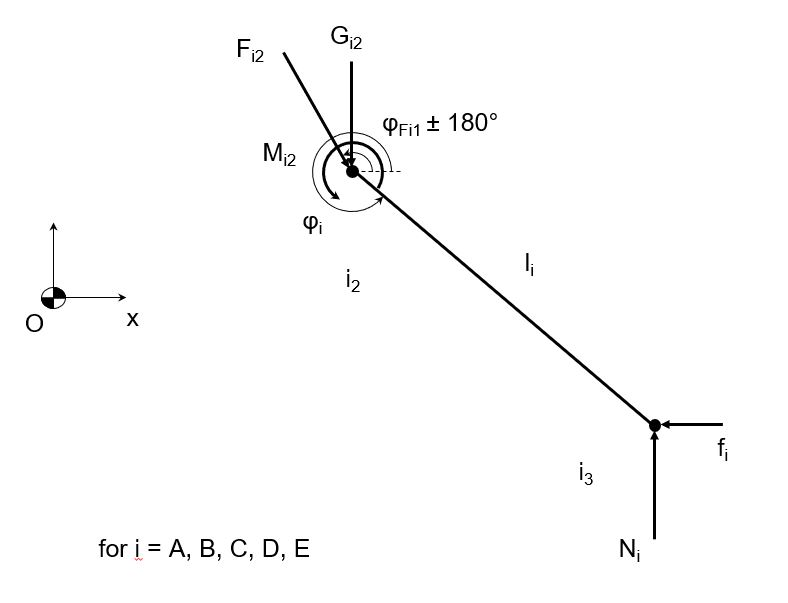
\includegraphics[width=0.8\textwidth]{4_ComponentProperties/img/robot_tibia_fbd.JPG}
    \caption{FBD of Tibia Member}
    \label{fig:robot_tibia_fbd}
\end{figure}

This allows the knee joint moment to be calculated using the following equation.

\begin{gather}
    \sum M_{i_2} = 0 = N_i l_i \cos{\phi_i} - M_{i_2}
    \\
    M_{i_2} = N_i l_i \cos{\phi_i}
\end{gather}

An example for the knee joint moment calculation of leg A, using the worst case normal force is as follows:
\begin{gather}
    \sum M_{A_2} = 0 = N_A l_A \cos{\phi_A} - M_{A_2}
    \\
    M_{A_2} = N_A l_A \cos{\phi_A} = (285 \text{N})(300 \text{mm})(\cos(315^{\circ})) = 60,423 \text{ Nmm}
\end{gather}

The forces acting on the leg (including the tibia and thigh members) are shown in Figure \ref{fig:robot_leg_fbd}.

\begin{figure}
    \centering
    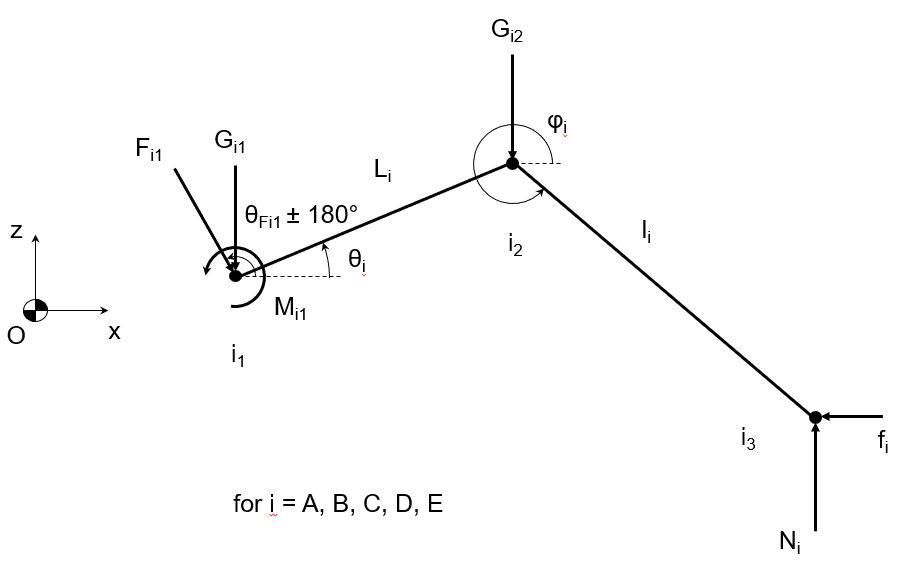
\includegraphics[width=0.8\textwidth]{4_ComponentProperties/img/robot_leg_fbd.JPG}
    \caption{FBD of Whole Leg}
    \label{fig:robot_leg_fbd}
\end{figure}

This allows the hip joint moment to be calculated using the following equation.

\begin{gather}
    \sum M_{i_1} = 0 = N_i [L_i \cos{\theta_i} + l_i \cos{\phi_i}] - G_{i2} L_i \cos{\theta_i} - M_{i_1}
    \\
    M_{i_1} = N_i [L_i \cos{\theta_i} + l_i \cos{\phi_i}] - G_{i2} L_i \cos{\theta_i}
\end{gather}

An example for the hip joint moment calculation of leg A, using the worst case normal force is as follows:

\begin{equation}
    \sum M_{A_1} = 0 = N_A [L_A \cos{\theta_A} + l_A \cos{\phi_A}] - G_{i2} L_A \cos{\theta_A} - M_{A_1}
\end{equation}

\begin{equation}
\begin{split}
        M_{A_1} = N_A [L_A \cos{\theta_A} + l_A \cos{\phi_A}] - G_{i2} L_A \cos{\theta_A} 
        \\
        = (285 \text{N})[(300 \text{mm}) \cos{(0^{\circ})} + (300 \text{mm}) \cos{(315^{\circ})}] - (0.282 \text{kg})g (300 \text{mm}) \cos{(0^{\circ})} 
        \\= 145, 048 \text{Nmm}
\end{split}
\end{equation}

Table \ref{tab:torques} shows the torque values obtained for two static calculation types. The first is when the normal forces are assumed to be a quarter of the robot weight (as if one leg is off the ground). The second is using the worst case method outlined previously where torques are calculated based on only three legs touching the ground. It can be seen that the highest torques appear in legs A and B. These are considered as determined in Section \ref{sec:ass_motors}.

\begin{table}[H]
    \centering
    \caption{Leg Joint Torques Based on Two Different Calculated Normal Forces}
    \label{tab:torques}
    \begin{tabular}{l c c c}
        \\ \hline
        \textbf{Method} & \textbf{Leg} & \textbf{Knee Torque [Nmm]} & \textbf{Hip Torque [Nmm]}
        \\ \hline
        Equal Normal Forces & All & 36,000 & 86,000
        \\
        Worst Case Normal Forces & A & 60,000 & 145,000
        \\
          & B & 60,000 & 145,000
        \\
         & C & 30,000 & 72,000
        \\
         & D & 41,000 & 100,000
        \\
         & E & 30,000 & 72,000
        \\ \hline
    \end{tabular}
\end{table}


%------------- JOINT TORQUES DYNAMIC EQUATION -------------%
\subsection{Generalized Dynamic Equation of Motion} \label{subsec:dynamic_equation}

For both the static dynamic case where the legs are moving, the joint torques can be found by developing an inertial matrix, force and gravity matrices, and using them in the dynamic equation developed in the Robotics course, MCG4134 \cite{al-jarrah_mcg4134:_2019}.
The final form, following derivations described in Appendix \ref{app:dynamic_equation} and for an arbitrary leg $i$ shown in Figure \ref{fig:dynamic_leg} with joint torques consistent with Figures \ref{fig:robot_tibia_fbd} and \ref{fig:robot_leg_fbd}, is equation \ref{eq:dynamic_equation}.

\begin{figure}[H]
    \centering
    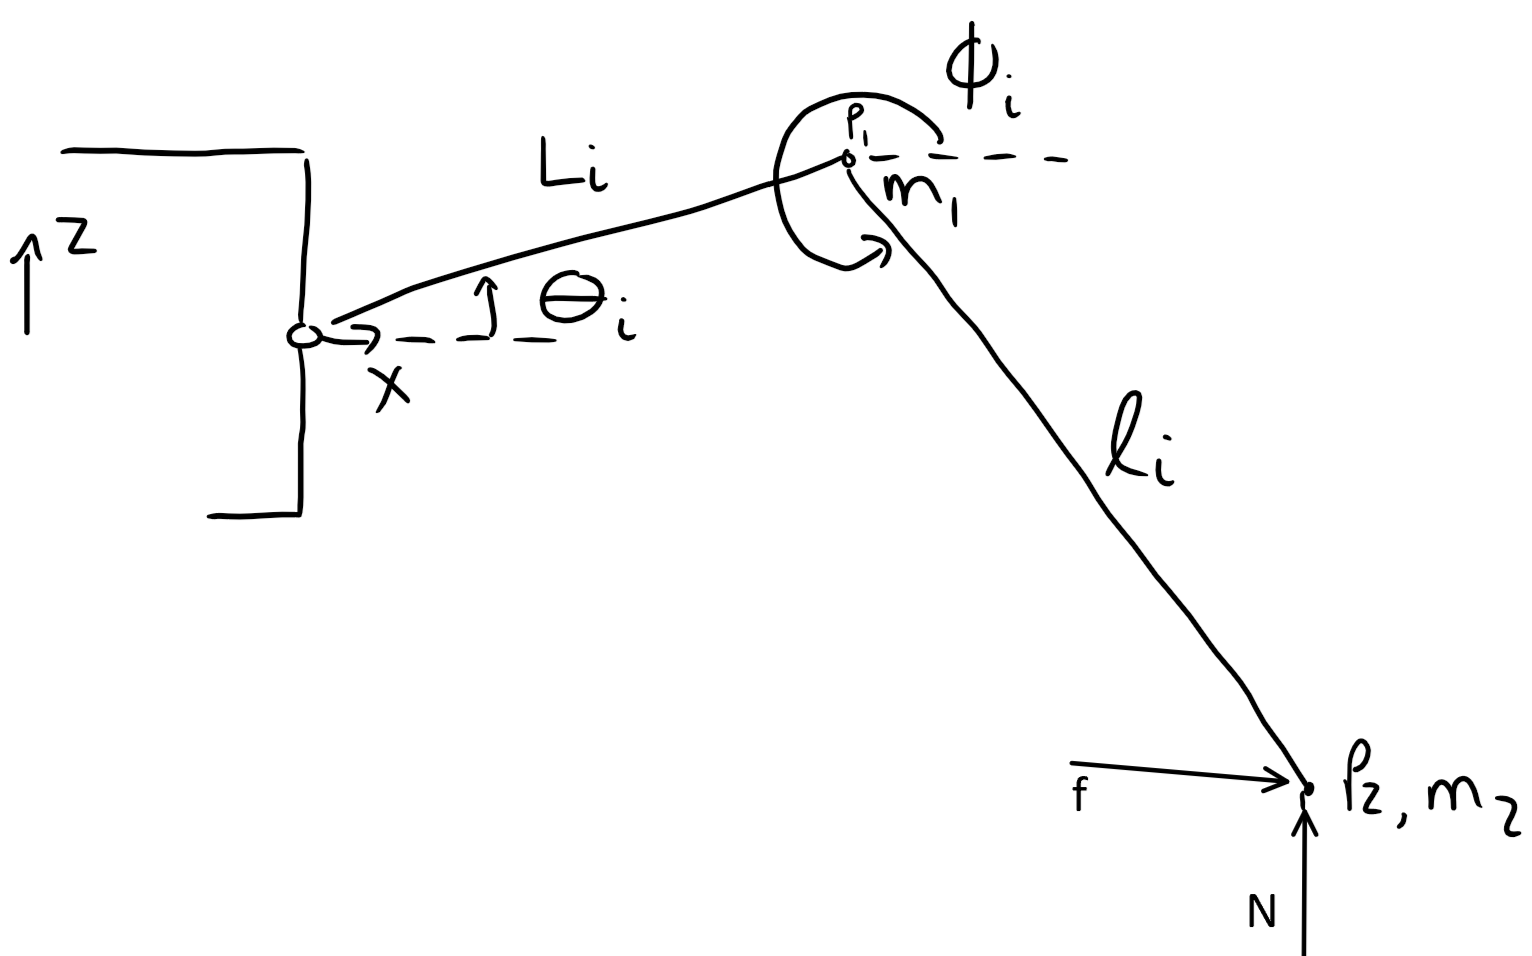
\includegraphics[width=0.6\textwidth]{5_KinematicAndForces/img/dynamic_leg.png}
    \caption{Side View of Leg $i$}
    \label{fig:dynamic_leg}
\end{figure}

\begin{equation} \label{eq:dynamic_equation}
    \begin{split}
        \begin{bmatrix} 
            (m_1 + m_2) L^2 & m_2 \ell L \cos(\theta-\phi) \\
            m_2 \ell L \cos(\theta-\phi) & m_2 \ell
        \end{bmatrix}
        \begin{bmatrix} \Ddot{\theta} \\ \Ddot{\phi} \end{bmatrix}
        +
        g \begin{bmatrix}
            (m_1 + m_2) L \cos\theta + m_2 \ell \cos\theta \\
            m_2 \ell \cos\phi
        \end{bmatrix} \\
        +
        N \begin{bmatrix}
            L\cos\theta + \ell\cos\phi \\
            \ell\cos\phi
            \end{bmatrix} + f \begin{bmatrix}
            L\sin\theta + \ell\sin\phi \\
            \ell\sin\phi
        \end{bmatrix}
        =
        \begin{bmatrix}
        \tau_1 \\ \tau_2
        \end{bmatrix}
    \end{split}
\end{equation}

where $m_1$ and $m_2$ are the masses of the linkages and joints (moved to the most distal point of the linkage), $N$ is the normal force at the foot, $f$ is the friction force at the foot (and encompasses wind, chassis acceleration, and other external forces parallel the ground), and $\tau_1$ and $\tau_2$ are the joint torques at the hip and knee respectively.
This approach is conservative, as the actual inertial matrix would contain mass values closer to the center of the linkages.
It also simplifies the mass moment of inertia calculations presented in Appendix \ref{app:mass_moment_of_inertia}.
An example with leg A is shown below, where the chassis was assumed to be accelerating forward at a rate of $a = 0.5m/s^2$ on a flat surface with no wind.
The maximum static friction force $f_{max} = \mu N$ is assumed to be superior to the reaction at the foot to allow for the chassis to move forward with $F = ma = f$ (no slipping).
Assuming an even distribution of load and three legs making contact with the ground, the friction force per leg is thus one third of the force required to move the the chassis.

\begin{equation}
    f = \frac{ma}{3} = \frac{(63\text{kg})(0.5m/s^2)}{3 \text{legs}} = 10.62 N
\end{equation}

\begin{equation} \label{eq:dynamic_equation_example}
    \begin{split}
        \begin{bmatrix} 
            (0.836 \text{kg} + 0.532 \text{kg}) (300 \text{mm})^2 & (0.532 \text{kg}) (300 \text{mm}) (300 \text{mm}) \cos(0^{\circ} - 315^{\circ}) \\
            0.532 \text{kg} (300 \text{mm}) (300 \text{mm}) \cos(0^{\circ} - 315^{\circ}) & 0.532 \text{kg} (300 \text{mm})
        \end{bmatrix} 
        \begin{bmatrix} (5 rad/s^2) \\ (5 rad/s^2) \end{bmatrix}\\
        +
        (9.81 m/s^2) \begin{bmatrix}
            (0.836 \text{kg} + 0.532 \text{kg}) (300 \text{mm}) \cos(0^{\circ}) + 0.532 \text{kg} (300 \text{mm}) \cos(0^{\circ}) \\
            m_2 (300 \text{mm}) \cos(315^{\circ})
        \end{bmatrix} \\
        +
        (285 \text{N}) \begin{bmatrix}
            (300 \text{mm})\cos(0^{\circ}) + (300 \text{mm})\cos(315^{\circ}) \\
            (300 \text{mm})\cos(315^{\circ})
            \end{bmatrix}
            \\+ (10.62 \text{N}) \begin{bmatrix}
           (300 \text{mm})\sin(0^{\circ}) + (300 \text{mm})\sin(315^{\circ}{}) \\
            (300 \text{mm})\sin(315^{\circ}{})
        \end{bmatrix}
        =
        \begin{bmatrix}
        (150,000 Nmm) \\ (60,000 Nmm)
        \end{bmatrix}
    \end{split}
\end{equation}

Tables \ref{tab:torques_Moving_forward} and \ref{tab:torques_Moving_backward} show the values obtained for all other leg following the same equation at the given acceleration, for both forward and backwards motion. Theses table can be compared with Table \ref{tab:torques}; all torques are very similar and very close in value.

\begin{table}[H]
    \centering
    \caption{Leg Joint Torque Based on Generalized Equation of Motion with Forward Acceleration}
    \label{tab:torques_Moving_forward}
    \begin{tabular}{l c c c}
        \\ \hline
        \textbf{Method} & \textbf{Leg} & \textbf{Knee Torque [Nmm]} & \textbf{Hip Torque [Nmm]}
        \\ \hline
        Generalized Equation of Motion & A & 60,000 & 149,000
        \\
          & B & 60,000 & 152,000
        \\
         & C & 33,000 & 80,000
        \\
         & D & 44,000 & 108,000
        \\
         & E & 33,000 & 80,000
        \\ \hline
    \end{tabular}
\end{table}

\begin{table}[H]
    \centering
    \caption{Leg Joint Torque Based on Generalized Equation of Motion with Backward Acceleration}
    \label{tab:torques_Moving_backward}
    \begin{tabular}{l c c c}
        \\ \hline
        \textbf{Method} & \textbf{Leg} & \textbf{Knee Torque [Nmm]} & \textbf{Hip Torque [Nmm]}
        \\ \hline
        Generalized Equation of Motion & A & 65,000 & 155,000
        \\
          & B & 65,000 & 155,000
        \\
         & C & 28,000 & 76,000
        \\
         & D & 40,000 & 104,000
        \\
         & E & 28,000 & 75,000
        \\ \hline
    \end{tabular}
\end{table}


%------------- Stability Analysis and Slopes -------------%
\subsection{Stability Analysis and Slopes}
\label{sec:stability}
The stability analysis allows to determine the area of stability of the robot. Stability triangles show the limit and area of stability of the robot when standing on three of the five legs. By linking legs in combinations as seen in section \ref{sec:normal_forces}, a stability diagram is created as shown in Figure \ref{fig:centreMass}. The centre of mass must be located at all times in the diamond shaped area located in the middle of the robot. This will ensure a constant stability with whichever combination of legs.

\begin{figure}[H]
    \centering
    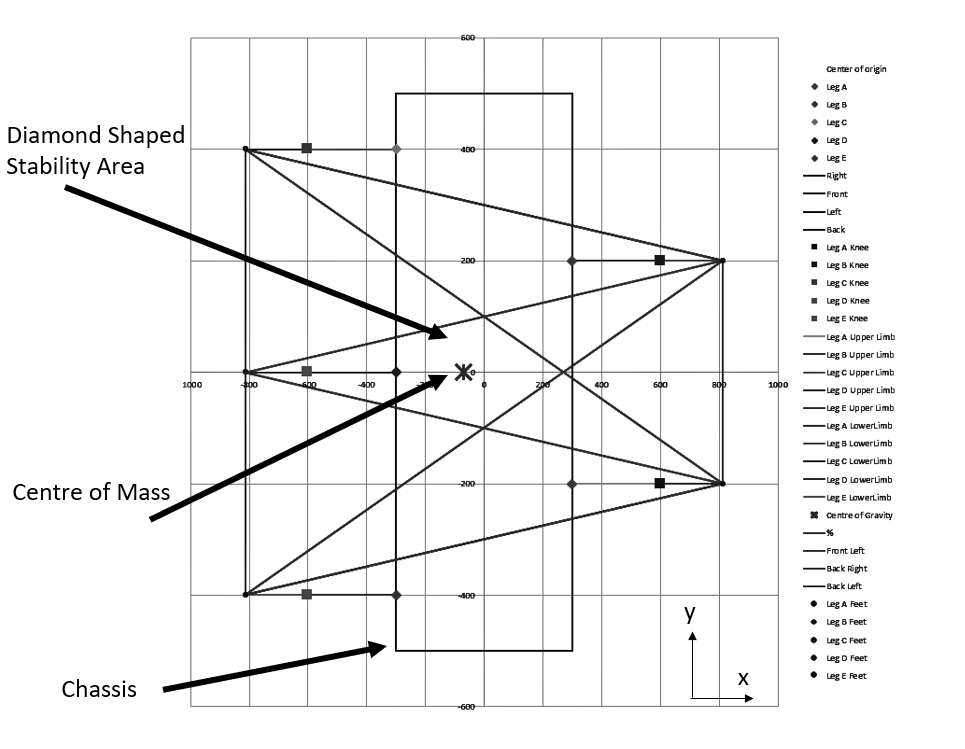
\includegraphics[width=\textwidth]{5_KinematicAndForces/img/CentreMass.PNG}
    \caption{Centre of Mass and Diamond Shaped Stability Area}
    \label{fig:centreMass}
\end{figure}

To assess the robots' stability on slopes, rotational matrices were used around X, Y, and Z \cite{al-jarrah_mcg4134:_2019}. These are shown here:
\begin{equation}
    R_x = \left[ \begin{array}{ccc} 
    1 & 0 & 0 
    \\ 
    0 & \cos\theta & -\sin\theta 
    \\ 
    0 & \sin\theta & \cos\theta
    \end{array} \right] 
\end{equation}
    
\begin{equation}
    R_y = \left[ \begin{array}{ccc} 
    \cos\phi & 0 & \sin\phi 
    \\ 
    0 & 1 & 0 
    \\ 
    -\sin\phi & 0 & \cos\phi
    \end{array} \right] 
\end{equation}
    
\begin{equation}
    R_z = \left[ \begin{array}{ccc} 
    \cos\sigma & -\sin\sigma & 0
    \\ 
    \sin\sigma & \cos\sigma & 0 
    \\ 
    0 & 0 & 1
    \end{array} \right] 
\end{equation}

The fixed frame's Z direction is always parallel and in the opposite direction to the gravitational force. The fixed frame is defined by $\left[ \begin{array}{ccc} X & Y & Z \end{array} \right]^{-1}$. The robot's frame is defined by $\left[ \begin{array}{ccc} x & y & z \end{array} \right]^{-1}$

Rotation from x to z $R_2^0$ is defined as:
\begin{equation}
    R_z^x = R_zR_yR_x
\end{equation}

Thus, to obtain the robot's location, the following equation is used:
\begin{equation} \label{eq:rotational matrix}
    \left[ \begin{array}{ccc} x \\ y \\ z \end{array} \right] = 
    R_z^x
    \left[ \begin{array}{ccc} X \\ Y \\ Z \end{array} \right]
\end{equation}

Using equation \ref{eq:rotational matrix}, it was possible to model every component of the robot according to the rotations. Using the stability triangles, the maximum slope angle can be determined. The  figures \ref{fig:rotation_20}, \ref{fig:rotation_-20}, \ref{fig:rotation_57}, \ref{fig:rotation_-73} shows the robot's center of mass at different locations depending on the slope. The center of mass is the star, which should always be located within the area of stability. It should be noted that the centre of mass itself is not moving, even though it looks like it on the images. The shift between the stability area and centre of mass is created due to their difference in height.

An example using the position of centre of mass is as follows at 20 degrees around x:

\begin{equation} \label{eq:rotational_matrix}
    \left[ \begin{array}{ccc} x \\ y \\ z \end{array} \right] = 
    \left[ \begin{array}{ccc} 1 & 0 & 0 \\ 0 & 0.940 & -0.342 \\ 0 & 0.342 & 0.940
    \end{array} \right]
    \left[ \begin{array}{ccc} 740 \text{mm} \\ 400 \text{mm} \\ 221 \text{mm} \end{array} \right] = \left[ \begin{array}{ccc} 740 \text{mm} \\ 300 \text {mm} \\ 344 \text {mm} \end{array} \right]
\end{equation}



\begin{figure} [H]
    \centering
    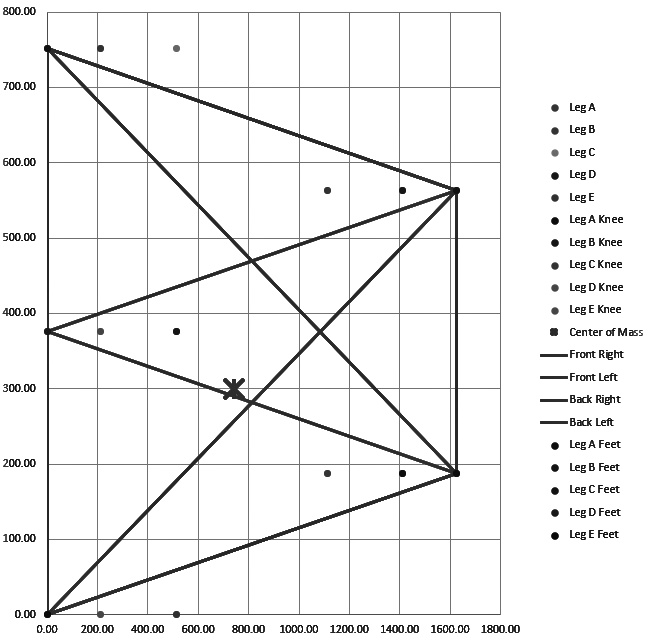
\includegraphics[width=\textwidth]{5_KinematicAndForces/img/CenterMass_20_X.PNG}
    \caption{Rotation Around X by 20\textdegree{}}
    \label{fig:rotation_20}
\end{figure}

\begin{figure} [H]
    \centering
    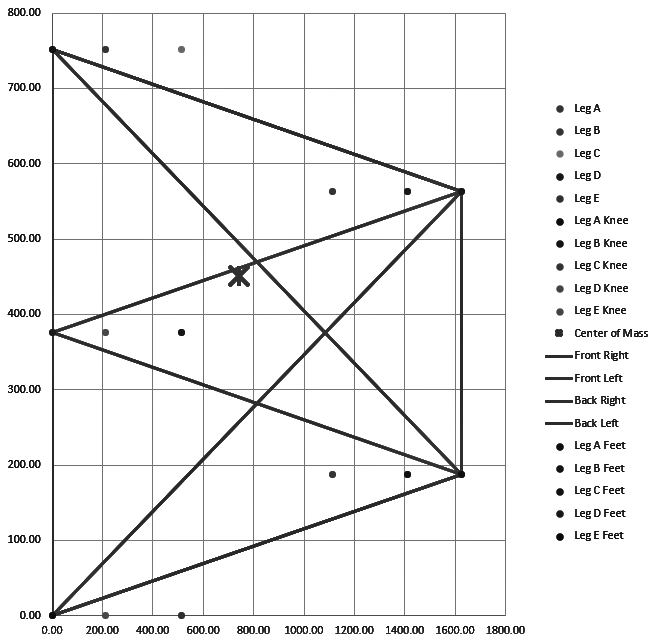
\includegraphics[width=\textwidth]{5_KinematicAndForces/img/CenterMass_-20_X.PNG}
    \caption{Rotation Around X by -20\textdegree{}}
    \label{fig:rotation_-20}
\end{figure}

\begin{figure} [H]
    \centering
    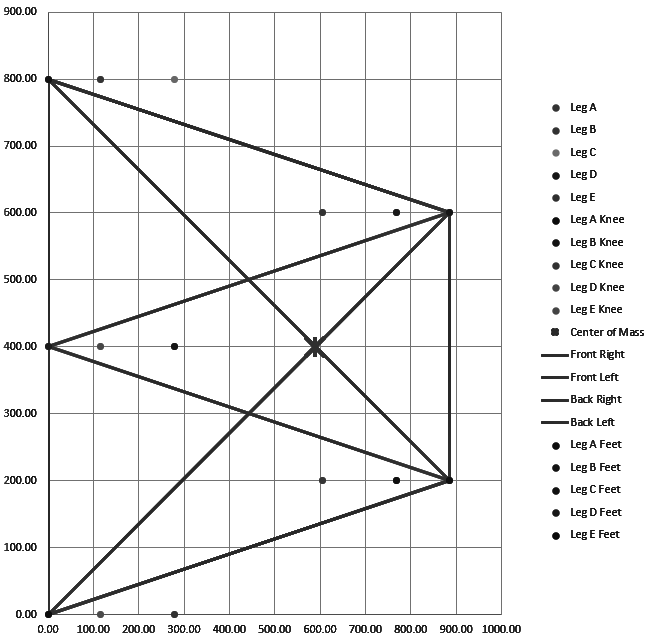
\includegraphics[width=\textwidth]{5_KinematicAndForces/img/CenterMass_57_Y.PNG}
    \caption{Rotation Around Y by 57\textdegree{}}
    \label{fig:rotation_57}
\end{figure}

\begin{figure} [H]
    \centering
    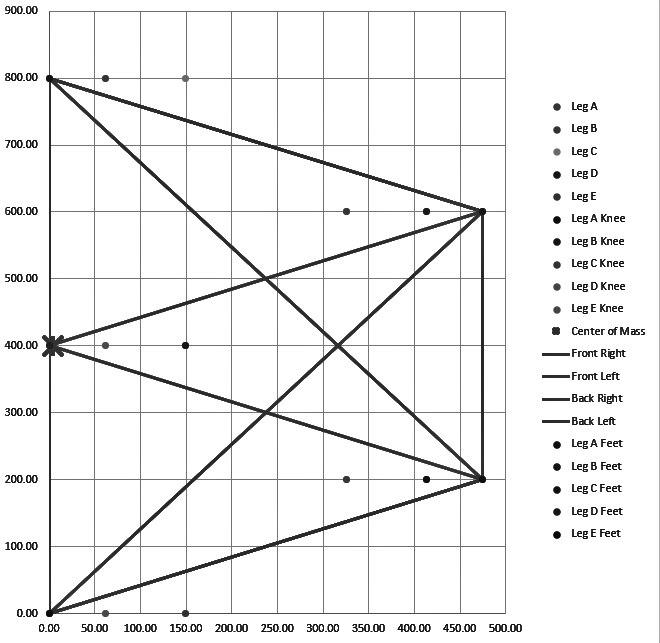
\includegraphics[width=\textwidth]{5_KinematicAndForces/img/CenterMass_-73_Y.PNG}
    \caption{Rotation Around Y by -73\textdegree{}}
    \label{fig:rotation_-73}
\end{figure}




%------------- Drag Force from Wind -------------%
\subsection{Drag Force from Wind} \label{subsec:wind}

Another external force to consider is the drag force acting on the robot from the wind. Strong winds are common on the waterfront and have the potential to flip the crab over if its weight is not sufficient to keep it on the ground. Based on last year's wind speed data, Ottawa experienced a maximum wind speed of 50 km/h (13.89 m/s) and a maximum gust of 73 km/h (20.78 m/s) in September 2018, which coincides with the tornadoes that occurred in the region \cite{weatherstats_wind_2019}. To calculate the drag force acting on the robot, the drag coefficient $C_{D}$ is obtained from Figure \ref{fig:drag_coef} in Appendix \ref{app:drag_coeff}. The value obtained is $C_{D} = 1.3$ based on the robot's width, depth, and height given in Table \ref{table:gen_dim}. For that case to be valid, the Reynold's number should be approximately $10^5$. The equation below is used to calculate the Reynold's number for wind velocity $U$ of $20.28 m/s$, a characteristic length $D$ (height $h$) of $0.2 m$, and a kinematic viscosity $\nu$ of $1.426x10^-5 m^2/s$ for air at 10\textdegree{}C and $1 atm$ \cite{munson_fundamentals_2009}\cite{engineers_edge_viscosity_2019}.

\begin{equation}
    Re = \frac{UD}{\nu} = \frac{(20.28 \text m/s)(0.2 \text m)}{1.426 \times 10^{-5} \text m^2/s } = 2.84 \times 10^{5}
\end{equation}

Since $2.84 \times 10^5$ has the same order of magnitude as $10^5$, the case used is assumed to be valid. Then, the drag force is calculated using the following equation \cite{munson_fundamentals_2009}.

\begin{equation} 
    F_D = \frac{1}{2}\rho U^2 C_D A = \frac{1}{2}(1.246 \text kg/m^3)(20.28 \text m/s)^2(1.3)(1 \text m)(0.2 \text m) = 66.62 \text N
\end{equation}

where $\rho$ is the density of the air at $10 ^{\circ} C$ and $A$ is the reference area of the chassis ($A = bD = wh$) \cite{engineers_edge_viscosity_2019}.

The worst case scenario for the robot with drag force is in the situation on a inclined slope of 20 degrees rotated with respect to the y axis as illustrated in Figure \ref{fig:crab_side_slope}. The drag force required to flip the robot is calculated using Figure \ref{fig:drag_worst_case}. The equations are as follows:

\begin{gather}
    d = -H\sin\theta + D\cos\theta = -(350 mm)\sin(20 \deg) + (300 mm)\cos(20\deg) = 162 mm
    \\
    h = H \cos\theta + D\sin\theta = (350 mm)\cos(20\deg) + (300 mm)\sin(20\deg) = 431 mm 
    \\
    \sum M = 0 = F_D h - mgd \xrightarrow{} F_D =  \frac{mgd}{h} \\
   F_D =  \frac{mgd}{h} = \frac{(63.6928 kg)(9.81 m/s^2)(256 mm)}{(468 mm)} = 235 N
\end{gather}

\begin{figure}
    \centering
    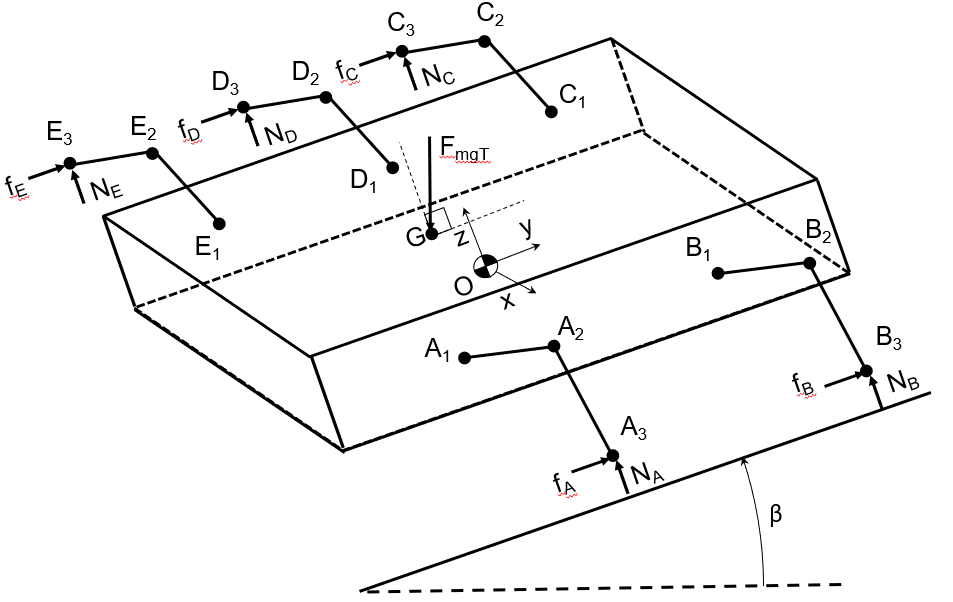
\includegraphics[width=0.9\textwidth]{4_ComponentProperties/img/robot_ext_fbd_slope_side.PNG}
    \caption{FBD of Whole Robot on a Slope}
    \label{fig:crab_side_slope}
\end{figure}

\begin{figure}
    \centering
    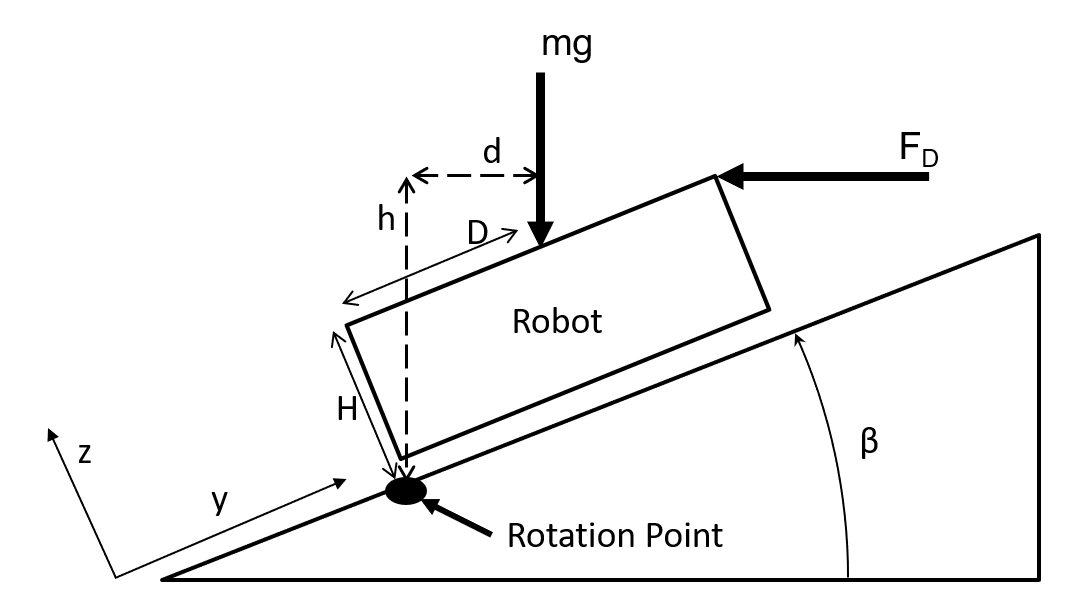
\includegraphics[width=\textwidth]{img/DragForce.png}
    \caption{Drag Force Worst Case Scenario}
    \label{fig:drag_worst_case}
\end{figure}